%
%Academic CV LaTeX Template
% Author: Dubasi Pavan Kumar
% LinkedIn: https://www.linkedin.com/in/im-pavankumar/
% License: MIT
%
% For errors, suggestions, or improvements, please contact:
% Email: pavankumard.pg19.ma@nitp.ac.in
%



\documentclass[letterpaper,11pt]{article}

% Package imports
\usepackage{latexsym}
\usepackage{xcolor}
\usepackage{float}
\usepackage{ragged2e}
\usepackage[empty]{fullpage}
\usepackage{wrapfig}
\usepackage{lipsum}
\usepackage{tabularx}
\usepackage{titlesec}
\usepackage{geometry}
\usepackage{marvosym}
\usepackage{verbatim}
\usepackage{enumitem}
\usepackage{fancyhdr}
\usepackage{multicol}
\usepackage{graphicx}
\usepackage{cfr-lm}
\usepackage[T1]{fontenc}
\usepackage{fontawesome5}
\usepackage{gensymb}%for the degree symbol

% Color definitions
\definecolor{darkblue}{RGB}{0,0,139}

% Page layout
\setlength{\multicolsep}{0pt}
\pagestyle{fancy}
\fancyhf{} % clear all header and footer fields
\fancyfoot{}
\renewcommand{\headrulewidth}{0pt}
\renewcommand{\footrulewidth}{0pt}
\geometry{left=1.4cm, top=0.8cm, right=1.2cm, bottom=1cm}
\setlength{\footskip}{5pt} % Addressing fancyhdr warning

% Hyperlink setup (moved after fancyhdr to address warning)
% Links are colored (not hidden) so readers can see what's clickable in the PDF
\usepackage{hyperref}
\hypersetup{
    colorlinks=true,
    linkcolor=darkblue,
    filecolor=darkblue,
    urlcolor=darkblue,
}

% Custom box settings
\usepackage[most]{tcolorbox}
\tcbset{
    frame code={},
    center title,
    left=0pt,
    right=0pt,
    top=0pt,
    bottom=0pt,
    colback=gray!20,
    colframe=white,
    width=\dimexpr\textwidth\relax,
    enlarge left by=-2mm,
    boxsep=4pt,
    arc=0pt,outer arc=0pt,
}

% URL style
\urlstyle{same}

% Text alignment
\raggedright
\setlength{\tabcolsep}{0in}

% Section formatting
\titleformat{\section}{
  \vspace{-4pt}\scshape\raggedright\large
}{}{0em}{}[\color{black}\titlerule \vspace{-7pt}]

% Custom commands
\newcommand{\resumeItem}[2]{
  \item{
    \textbf{#1}{\hspace{0.5mm}#2 \vspace{-0.5mm}}
  }
}

\newcommand{\resumePOR}[3]{
\vspace{0.5mm}\item
    \begin{tabular*}{0.97\textwidth}[t]{l@{\extracolsep{\fill}}r}
        \textbf{#1}\hspace{0.3mm}#2 & \textit{\small{#3}}
    \end{tabular*}
    \vspace{-2mm}
}

\newcommand{\resumeSubheading}[4]{
\vspace{0.5mm}\item
    \begin{tabular*}{0.98\textwidth}[t]{l@{\extracolsep{\fill}}r}
        \textbf{#1} & \textit{\footnotesize{#4}} \\
        \textit{\footnotesize{#3}} &  \footnotesize{#2}\\
    \end{tabular*}
    \vspace{-2.4mm}
}

% Education entry: {institution}{location}{degree}{date}{GPA}
% GPA sits right-aligned under the location instead of taking its own bullet line
\newcommand{\resumeEducation}[5]{
\vspace{0.5mm}\item
    \begin{tabular*}{0.98\textwidth}[t]{l@{\extracolsep{\fill}}r}
        \textbf{#1} & \textit{\footnotesize{#4}} \\
        \textit{\footnotesize{#3}} & \footnotesize{\begin{tabular}[t]{@{}r@{}}#2\\#5\end{tabular}}\\
    \end{tabular*}
    \vspace{-1mm}
}

\newcommand{\resumeProject}[4]{
\vspace{0.5mm}\item
    \begin{tabular*}{0.98\textwidth}[t]{l@{\extracolsep{\fill}}r}
        \textbf{#1} & \textit{\footnotesize{#3}} \\
        \footnotesize{\textit{#2}} & \footnotesize{#4}
    \end{tabular*}
    \vspace{-2.4mm}
}

% Reference entry: {name}{title}{institution}{email}{phone}{relationship}
% Compact 3-line form; \newline (not \\) because it sits inside a tabularx cell
\newcommand{\resumeReference}[6]{%
\textbf{#1} \textit{(#6)}\newline
#2, #3\newline
\href{mailto:#4}{#4} | #5%
}

\newcommand{\resumeSubItem}[2]{\resumeItem{#1}{#2}\vspace{-4pt}}

\renewcommand{\labelitemi}{$\vcenter{\hbox{\tiny$\bullet$}}$}
\renewcommand{\labelitemii}{$\vcenter{\hbox{\tiny$\circ$}}$}

\newcommand{\resumeSubHeadingListStart}{\begin{itemize}[leftmargin=*,labelsep=1mm]}
\newcommand{\resumeHeadingSkillStart}{\begin{itemize}[leftmargin=*,itemsep=1.7mm, rightmargin=2ex]}
\newcommand{\resumeItemListStart}{\begin{itemize}[leftmargin=*,labelsep=1mm,itemsep=0.5mm]}

\newcommand{\resumeSubHeadingListEnd}{\end{itemize}\vspace{2mm}}
\newcommand{\resumeHeadingSkillEnd}{\end{itemize}\vspace{-2mm}}
\newcommand{\resumeItemListEnd}{\end{itemize}\vspace{-2mm}}
\newcommand{\cvsection}[1]{%
\vspace{2mm}
\begin{tcolorbox}
    \textbf{\large #1}
\end{tcolorbox}
    \vspace{-4mm}
}

\newcolumntype{L}{>{\raggedright\arraybackslash}X}%
\newcolumntype{R}{>{\raggedleft\arraybackslash}X}%
\newcolumntype{C}{>{\centering\arraybackslash}X}%

% Commands for icon sizing and positioning
\newcommand{\socialicon}[1]{\raisebox{-0.05em}{\resizebox{!}{1em}{#1}}}
\newcommand{\ieeeicon}[1]{\raisebox{-0.3em}{\resizebox{!}{1.3em}{#1}}}

% Font options
\newcommand{\headerfonti}{\fontfamily{phv}\selectfont} % Helvetica-like (similar to Arial/Calibri)
\newcommand{\headerfontii}{\fontfamily{ptm}\selectfont} % Times-like (similar to Times New Roman)
\newcommand{\headerfontiii}{\fontfamily{ppl}\selectfont} % Palatino (elegant serif)
\newcommand{\headerfontiv}{\fontfamily{pbk}\selectfont} % Bookman (readable serif)
\newcommand{\headerfontv}{\fontfamily{pag}\selectfont} % Avant Garde-like (similar to Trebuchet MS)
\newcommand{\headerfontvi}{\fontfamily{cmss}\selectfont} % Computer Modern Sans Serif
\newcommand{\headerfontvii}{\fontfamily{qhv}\selectfont} % Quasi-Helvetica (another Arial/Calibri alternative)
\newcommand{\headerfontviii}{\fontfamily{qpl}\selectfont} % Quasi-Palatino (another elegant serif option)
\newcommand{\headerfontix}{\fontfamily{qtm}\selectfont} % Quasi-Times (another Times New Roman alternative)
\newcommand{\headerfontx}{\fontfamily{bch}\selectfont} % Charter (clean serif font)

\begin{document}
\headerfontiii

% Header
\begin{center}
    {\Huge\textbf{Mitchell Tillman, PhD}}
\end{center}
\vspace{-6mm}

\begin{center}
    \small{
    +1-847-687-3787 | \href{mailto:mtillman14@gmail.com}{mtillman14@gmail.com}
    }
\end{center}
\vspace{-6mm}

\begin{center}
    \small{
    \socialicon{\faGlobe} \href{https://www.mitchelltillman.com}{mitchelltillman.com} |
    \socialicon{\faLinkedin} \href{https://www.linkedin.com/in/mitchelltillman/}{mitchelltillman} |
    \socialicon{\faGithub} \href{https://github.com/mtillman14}{mtillman14} |
    \ieeeicon{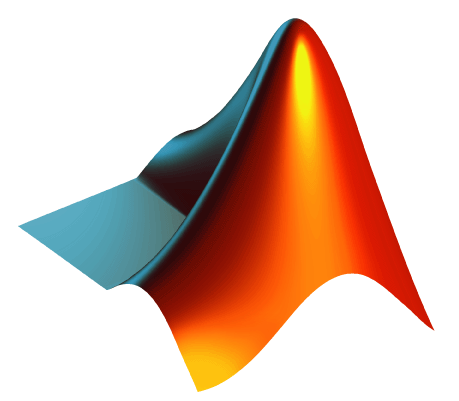
\includegraphics[height=1.3em]{matlab_icon.png}} \href{https://www.mathworks.com/matlabcentral/profile/authors/16297861}{Mitchell Tillman}
    }
\end{center}
\vspace{-6mm}
\begin{center}
    \small{Chicago, IL USA 60610}
\end{center}

\vspace{-4mm}

\section{\textbf{Objective}}
\vspace{1mm}
% \small{
Ph.D. seeking a data science position to leverage my academic research experience deriving actionable insights from complex datasets. I am passionate about developing tools to facilitate new discoveries in biomedical data.
}
% \small{
Seeking a sports biomechanist position, leveraging my expertise in analyzing human movement. Aiming to contribute to innovative projects at the intersection of biomechanics, motor control, and data science with the goal of improving movement performance. I am passionate about developing tools to facilitate new discoveries in biomechanical data, and I'm looking to grow my analytical skills and translate them to player development.
}
% \small{
Seeking a challenging position in biomechanics to leverage my expertise in analyzing human movement. Aiming to contribute to innovative projects at the intersection of biomechanics, motor control, data science, and practical problem-solving with the goal of improving movement performance. I am passionate about developing tools to facilitate new discoveries in biomechanical data, and I'm looking to learn more about data science practices in a production setting.
}
% \small{
Ph.D. in biomedical engineering seeking a challenging post-doctoral research position. Aiming to contribute to innovative projects at the intersection of biomechanics, motor control, data science, and practical problem-solving with the goal of improving movement rehabilitation and performance. I am also passionate about developing tools to facilitate new discoveries in biomechanical data.
}
% \small{
Ph.D. in biomedical engineering seeking a challenging and rewarding role as a biomechanist. My Ph.D. focused on the whole-body biomechanics of gait, and I aim to leverage that training to improve patients' quality of life. I am also passionate about developing tools to facilitate new discoveries in biomechanical data.
}
\small{
Postdoctoral fellow seeking a fee-for-service clinical biomechanist role, where patient-facing assessment and data analysis go hand in hand. My postdoc has combined delivering tSCS in the Tech Immersion clinic with device selection, rollout monitoring, and outcomes analysis for its hospital-wide implementation, building on Ph.D. training in whole-body gait biomechanics. My vision is for data to empower movement.
}

% \small{
Ph.D. in Biomedical Engineering with extensive experience in data analysis and statistical modeling seeking to join Abbott as a Staff Data Scientist. Aiming to leverage expertise in Python, R, and data analysis to contribute to the optimization of medical devices in diabetes care.
}
\vspace{-2mm}

\section{\textbf{Experience}}
\vspace{-0.4mm}
\resumeSubHeadingListStart

\resumeSubheading
  {Shirley Ryan AbilityLab}{Chicago, IL USA}
  {Postdoctoral Research Fellow, Center for Bionic Medicine}{2024 -- Present}
\resumeItemListStart
  \item Study the effects of transcutaneous spinal cord stimulation (tSCS) on gait in people with stroke and traumatic brain injury in Dr. Arun Jayaraman's lab
  \item Provide technical expertise to the Tech Immersion clinic, collecting and analyzing sensor data (EMG, IMU) to inform care for medically complex patients, and delivering tSCS treatment to spinal cord injury patients
  \item Contribute to implementing tSCS as hospital-wide standard clinical practice for spinal cord injury patients through stimulator device selection, rollout monitoring via analysis of clinical data pulls, outcomes analysis, and clinician education
  \item Co-authored three journal articles in 2026, including a first-author article in \textit{Neuromodulation}
\resumeItemListEnd

\resumeSubheading
  {Stevens Institute of Technology}{Hoboken, NJ USA}
  {Graduate Research Assistant, MSKCD Lab}{2019 -- 2024}
\resumeItemListStart
  \item Dissertation research with Dr. Antonia Zaferiou quantifying balance and momentum control during 90\degree~turns while walking in healthy young and older adults
  \item Collected motion capture and force plate data on over 50 young and older adult participants walking and turning
  \item Developed a MATLAB data analysis pipeline for custom analyses based on person-specific biomechanical models, including bespoke visualizations and data-driven videos. Designed the pipeline to handle large data volumes by minimizing the data held in memory
  \item Led three first-author journal articles from experiment design through data analysis and manuscript writing
\resumeItemListEnd

\resumeSubheading
  {Purdue University}{West Lafayette, IN USA}
  {Research Assistant, Biomechanics Lab}{2016 -- 2018}
\resumeItemListStart
  \item Studied how anticipation affects stability in finger force-production tasks with Dr. Satyajit Ambike, acquiring force transducer data and analyzing movement variability; first-authored three journal articles
\resumeItemListEnd

\resumeSubHeadingListEnd
\vspace{-6mm}

\section{\textbf{Projects}}
\vspace{-0.4mm}
\resumeSubHeadingListStart

\resumeProject
  {SciStack: Scientific data processing infrastructure (beta)}
  {Tools: Python, MATLAB, DuckDB, VS Code extension}
  {Sep 2021 -- Present}
  {{}\href{https://github.com/mtillman14/scistack}{\textcolor{darkblue}{\faGithub}}}
\resumeItemListStart
  \item Open-source framework providing the infrastructure to power researchers' existing Python or MATLAB analysis functions, so researchers can focus more on their science, and less on the code around the science
  \item Unique approach saves all data with its provenance (function, inputs, and settings), tracking settings and data versions instead of overwriting old results.
  \item Supports Python and MATLAB, even in the same project
  \item Implements common quality-of-life and time-saving features like missing data inventories, excluding outlier data, an auditable trail tracing a result back to the data it came from
  \item VS Code extension shows the pipeline as an interactive diagram with run controls, plotting, and statistics all built-in.
\resumeItemListEnd

\resumeProject
  {Real-time auditory biofeedback to assist balance}
  {Tools: MATLAB, OptiTrack motion capture, MaxMSP, Open Sound Control; Python, DeepLabCut Live}
  {2019 -- 2022}
  {}
\resumeItemListStart
  \item \textbf{Markered motion capture:} Developed the first prototype of a real-time marker-based motion capture auditory biofeedback system ($\sim$20 ms latency). 3 of 5 young adults improved one-legged standing balance in pilot testing
  % \item Tested older adults' understanding and device usability qualitatively with surveys and interviews
  \item \textbf{Markerless motion capture} Led a team of 10 high school students (\href{https://www.govstemscholars.com/scholars}{NJ Governor's STEM Scholars}, 2021 -- 2022) in developing a low-cost version using free software, mentored by Dr. Gary Kane, a core developer of DeepLabCut Live
\resumeItemListEnd

% \resumeProject
%   {Split-belt treadmill symmetry index return to baseline calculations}
%   {Tools: MATLAB}
%   {}
%   {}
% \resumeItemListStart
%   \item I analyzed the "symmetry index" data (measures left and right step length similarity) that Dr. Ray Lin at Seton Hall University collected on older adults walking on a split-belt treadmill
%   \item My responsibilities were to identify the features in the symmetry index timeseries to establish when the left and right belt speeds diverged, and to quantify how many steps it took for the symmetry index to return to plateau
% \resumeItemListEnd

\resumeSubHeadingListEnd

\section{\textbf{Education}}
\vspace{-0.4mm}
\resumeSubHeadingListStart

\resumeEducation
{Stevens Institute of Technology}{Hoboken, NJ USA}
{\parbox[t]{0.7\linewidth}{Ph.D. Mechanics of Whole-Body Balance and Momentum Control During \newline Straight-Line Gait and 90\degree~Turns}}{Oct 2024}{GPA: 4.00/4.00}

\resumeEducation
{Purdue University}{West Lafayette, IN USA}
{\parbox[t]{0.8\linewidth}{M.S. Effects of Past and Future Motor Events on Present Motor Stability, \newline and Relationships with Motor and Cognitive Flexibility}}{May 2019}{GPA: 3.59/4.00}

\resumeEducation
{Purdue University}{West Lafayette, IN USA}
{B.S. Movement \& Sports Sciences}{May 2018}{GPA: 3.12/4.00}

\resumeSubHeadingListEnd
\vspace{-6mm}

\section{\textbf{Selected Publications}}
\vspace{0.2mm}
\small{
\begin{enumerate}[leftmargin=*, labelsep=0.5em, align=left, widest={[\textbf{S.1}]}, itemindent=0em, label={\textbf{[\arabic*]}]}]
\item[\textbf{[1]}] \textbf{Tillman M}, et al. (2026). \href{https://doi.org/10.1016/j.neurom.2026.09.018}{\textbf{Acute effects of transcutaneous spinal cord stimulation (tSCS) on gait symmetry in people with chronic stroke}}. \textit{Neuromodulation}

\item[\textbf{[2]}] Kishta A, Khazanchi R, Veit N, \textbf{Tillman M}, et al. (2026). \href{https://doi.org/10.1159/000552236}{\textbf{Multimodal machine learning to personalize transcutaneous spinal cord stimulation for stroke rehabilitation}}. \textit{Digital Biomarkers}

\item[\textbf{[3]}] Veit NC, et al., \textbf{Tillman M}, et al. (2026). \href{https://doi.org/10.1152/jn.00500.2025}{\textbf{The effects of electrode configuration and location on motor thresholds, tolerance, and muscle selectivity of transcutaneous spinal cord stimulation in stroke}}. \textit{J. Neurophysiol.}

\item[\textbf{[4]}] \textbf{Tillman M}, et al. (2024). \href{https://doi.org/10.1186/s12984-024-01437-3}{\textbf{Healthy older adults generate transverse-plane momenta required for 90 degree turns during the same phases of gait as in straight-line gait}}. \textit{J. NeuroEng. Rehabil.}, 21:145

% \item[\textbf{[5]}] \textbf{Tillman M}, et al. (2020). \href{https://dl.acm.org/doi/10.1145/3401956.3404244}{\textbf{Real-time optical motion capture balance sonification system}}. \textit{ACM Int. Conf. Proc. Series}

% \item[\textbf{[5]}] \textbf{Tillman M}, et al. (2022). \href{https://doi.org/10.1016/j.jbiomech.2022.111206}{\textbf{Frontal plane balance during pre-planned and late-cued 90 degree turns while walking}}. \textit{J. Biomech.}

% \item[\textbf{[5]}] \textbf{Tillman M}, et al. (2018). \href{https://doi.org/10.1007/s00221-018-5333-0}{\textbf{Expectation of movement generates contrasting changes in multifinger synergies in young and older adults}}. \textit{Exp. Brain Res.}
\end{enumerate}
Full publication list: \href{https://www.mitchelltillman.com/publications/}{mitchelltillman.com/publications}
}

\section{\textbf{Skills}}
\vspace{-0.4mm}
 \resumeHeadingSkillStart
  \resumeSubItem{Programming Languages (in order of experience):}
    {MATLAB, Python, R, SQL, bash}
  \resumeSubItem{Databases \& Version Control:}
    {SQLite, DuckDB, Git, GitHub}
  \resumeSubItem{Statistics:}
    {Regression, ANOVA, k-means cluster analysis, linear mixed models}
  \resumeSubItem{Lab \& Clinical Technology:}
    {OptiTrack motion capture, force plates, transcutaneous spinal cord stimulation (tSCS), electromyography (Delsys), inertial measurement units (XSENS), DeepLabCut (markerless motion capture), DeepLabCut Live, MaxMSP}
  \resumeSubItem{Research, Clinical \& Leadership:}
    {Experiment design, research study management, team management, data collection, working with patients, clinical data analysis, clinically-relevant analyses, pipeline development, biomechanics}
 \resumeHeadingSkillEnd

\section{\textbf{Honors and Awards}}
\vspace{-0.4mm}
\resumeSubHeadingListStart

\resumeProject
  {Doctoral Excellence Fellowship}
  {Stevens Institute of Technology -- Full tuition and stipend for one academic year}
  {May 2023}
  {}

% \resumeProject
%   {Robert Crooks Stanley Fellowship}
%   {Robert Crooks Stanley Graduate Fellowship Committee}
%   {Aug 2022}
%   {{}\href{https://www.stevens.edu/academics/graduate-study/graduate-funding/assistantships-and-fellowships\#scholarships-fellowships}{\textcolor{darkblue}{\faIcon{globe}}}}
% \resumeItemListStart
%   \item Awarded to researchers exhibiting the qualities of industrialism upheld by the committee
% \resumeItemListEnd

\resumeProject
  {Outstanding Masters Student in the College of Health and Human Sciences}
  {Purdue University -- \$500 for outstanding achievements in original research}
  {May 2019}
  {}

\resumeSubHeadingListEnd

\vspace{-6mm}

\section{\textbf{Volunteer Experience}}
\vspace{-0.4mm}
\resumeSubHeadingListStart
\resumeProject
  {Student Committee Member}
  {American Society of Biomechanics (ASB)}
  {2022 -- 2024}
  {{}\href{https://asbweb.org}{\textcolor{darkblue}{\faIcon{globe}}}}
\resumeItemListStart
  \item Helped plan student sessions at the international ASB conference and secured \$5,000 sponsorship from OptiTrack two years running for the student night out
\resumeItemListEnd

\resumeProject
  {Secretary, Graduate Biomedical Engineering Society}
  {Stevens Institute of Technology}
  {Aug 2021 -- Aug 2022}
  {{}\href{https://ducklink.stevens.edu/gbmes/home/}{\textcolor{darkblue}{\faIcon{globe}}}}
\resumeItemListStart
  \item Instituted biweekly graduate student-led department seminars that are still ongoing
  \item Hosted career development events for the BME department, including negotiating funding from the school for food and external speakers
\resumeItemListEnd

% \resumeProject
%   {National Biomechanics Day}
%   {The Biomechanics Initiative at Stevens Institute of Technology}
%   {2020 -- 2023}
%   {{}\href{https://thebiomechanicsinitiative.org}{\textcolor{darkblue}{\faIcon{globe}}}}
% \resumeItemListStart
%   \item Introduced middle and high school students to biomechanics through interactive activities, such as dancing with EMG sensors to visualize muscle activity
% \resumeItemListEnd

\resumeSubHeadingListEnd
\vspace{-6mm}

% \section{\textbf{Professional Memberships}}
% \vspace{-0.4mm}
% \resumeSubHeadingListStart
% \resumePOR{American Society of Biomechanics}
%     {}
%     {2017 -- 2024}
% \resumePOR{International Society of Posture \& Gait Research}
%     {}
%     {2023 -- 2024}
% \resumePOR{Graduate Biomedical Engineering Society}
%     {}
%     {2021 -- 2022}
% \resumePOR{Society for Neuroscience}
%     {}
%     {2019, 2023}
% \resumeSubHeadingListEnd
% \vspace{-6mm}

\section{\textbf{References}}
\vspace{-0.2mm}
\footnotesize{
\begin{tabularx}{\textwidth}{@{}LL@{}}
\resumeReference{Dr. Antonia Zaferiou}
  {Assistant Professor, Biomedical Engineering}
  {Stevens Institute of Technology}
  {antonia.zaferiou@stevens.edu}{+1-201-216-3662}{Ph.D. Supervisor}
&
\resumeReference{Dr. Satyajit Ambike}
  {Associate Professor, Health \& Kinesiology}
  {Purdue University}
  {sambike@purdue.edu}{+1-614-209-8407}{M.S. Supervisor}
\\[2mm]
\resumeReference{Dr. Sean Sanford}
  {Senior Test Engineer}
  {Medtronic}
  {sean.sanford2@medtronic.com}{+1-480-824-8167}{Former Colleague}
&
\resumeReference{Nathaniel Bechhofer}
  {CEO}
  {FormToFile}
  {nathanielbechhofer@trovbase.com}{+1-845-570-1518}{Mentor and Industry Collaborator}
\end{tabularx}
}

\end{document}
